\definecolor{initColor}{RGB}{137,135,129}
\definecolor{finalColor}{RGB}{42,120,214}
\definecolor{trainColor}{RGB}{27,175,122}
\definecolor{valColor}{RGB}{235,104,52}
\begin{figure}[htbp]
\centering
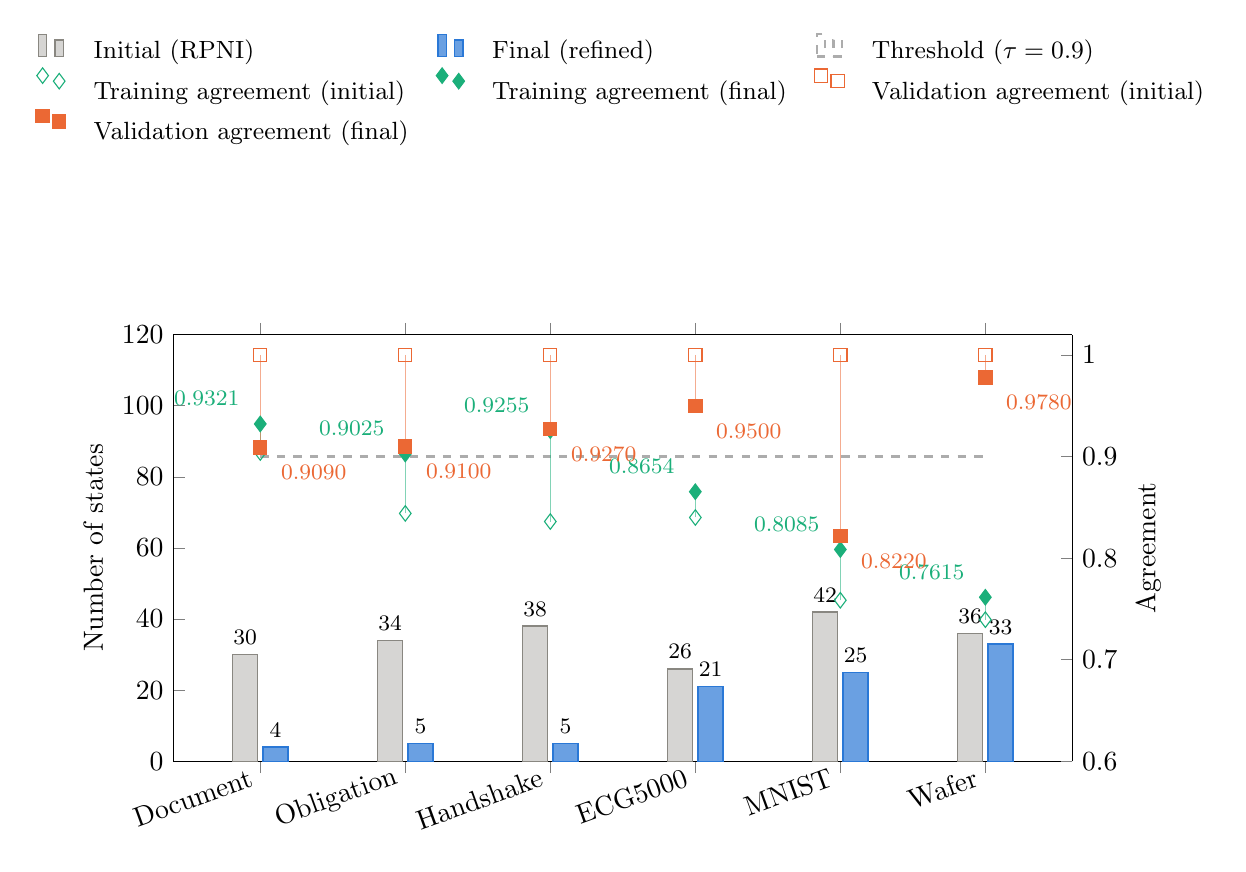
\begin{tikzpicture}
% ===== Left axis: initial and final states =====
% Carries the ONE combined legend for both axes: two overlaid axes each
% positioning their own legend via `at=` fight over the same coordinate
% space and silently clobber each other, so the right axis's series get
% phantom \addlegendimage entries here instead of a legend of their own.
\begin{axis}[
    width=13cm, height=7cm,
    ybar,
    bar width=9pt,
    axis y line*=left,
    ylabel={Number of states},
    ymin=0, ymax=120,
    symbolic x coords={Document,Obligation,Handshake,ECG5000,MNIST,Wafer},
    xtick=data,
    x tick label style={rotate=20, anchor=east},
    enlarge x limits=0.12,
    legend style={at={(0.5,1.42)}, anchor=south, legend columns=3, draw=none, font=\small, column sep=8pt},
    legend cell align=left,
    nodes near coords,
    every node near coord/.append style={font=\footnotesize},
]
\addplot[fill=initColor!35!white, draw=initColor, line width=0.5pt] coordinates {(Document,30) (Obligation,34) (Handshake,38) (ECG5000,26) (MNIST,42) (Wafer,36)};
\addlegendentry{Initial (RPNI)}
\addplot[fill=finalColor!70!white, draw=finalColor, line width=0.5pt] coordinates {(Document,4) (Obligation,5) (Handshake,5) (ECG5000,21) (MNIST,25) (Wafer,33)};
\addlegendentry{Final (refined)}
\addlegendimage{gray!65, dashed, line width=0.8pt}
\addlegendentry{Threshold ($\tau=0.9$)}
\addlegendimage{only marks, color=trainColor, mark=diamond, mark size=2.8pt}
\addlegendentry{Training agreement (initial)}
\addlegendimage{only marks, color=trainColor, mark=diamond*, mark size=2.8pt}
\addlegendentry{Training agreement (final)}
\addlegendimage{only marks, color=valColor, mark=square, mark size=2.4pt}
\addlegendentry{Validation agreement (initial)}
\addlegendimage{only marks, color=valColor, mark=square*, mark size=2.4pt}
\addlegendentry{Validation agreement (final)}
\end{axis}

% ===== Right axis: training / validation agreement, before vs. after =====
% Hollow marker = initial (origin RPNI automaton), filled marker = final
% (after refinement); the thin connecting segment makes the before/after
% change at each task read the same way the states bars do on the left axis.
\begin{axis}[
    width=13cm, height=7cm,
    axis y line*=right,
    axis x line=none,
    ylabel={Agreement},
    ymin=0.6, ymax=1.02,
    symbolic x coords={Document,Obligation,Handshake,ECG5000,MNIST,Wafer},
    xtick=data,
    enlarge x limits=0.12,
]
\addplot[color=gray!65, dashed, line width=0.8pt, forget plot]
    coordinates {(Document,0.9) (Wafer,0.9)};
\addplot[trainColor, thin, opacity=0.55, forget plot] coordinates {(Document,0.9040) (Document,0.9321)};
\addplot[trainColor, thin, opacity=0.55, forget plot] coordinates {(Obligation,0.8440) (Obligation,0.9025)};
\addplot[trainColor, thin, opacity=0.55, forget plot] coordinates {(Handshake,0.8360) (Handshake,0.9255)};
\addplot[trainColor, thin, opacity=0.55, forget plot] coordinates {(ECG5000,0.8400) (ECG5000,0.8654)};
\addplot[trainColor, thin, opacity=0.55, forget plot] coordinates {(MNIST,0.7585) (MNIST,0.8085)};
\addplot[trainColor, thin, opacity=0.55, forget plot] coordinates {(Wafer,0.7394) (Wafer,0.7615)};
\addplot[valColor, thin, opacity=0.55, forget plot] coordinates {(Document,1.0000) (Document,0.9090)};
\addplot[valColor, thin, opacity=0.55, forget plot] coordinates {(Obligation,1.0000) (Obligation,0.9100)};
\addplot[valColor, thin, opacity=0.55, forget plot] coordinates {(Handshake,1.0000) (Handshake,0.9270)};
\addplot[valColor, thin, opacity=0.55, forget plot] coordinates {(ECG5000,1.0000) (ECG5000,0.9500)};
\addplot[valColor, thin, opacity=0.55, forget plot] coordinates {(MNIST,1.0000) (MNIST,0.8220)};
\addplot[valColor, thin, opacity=0.55, forget plot] coordinates {(Wafer,1.0000) (Wafer,0.9780)};
\addplot[only marks, color=trainColor, mark=diamond, mark size=2.8pt, forget plot]
    coordinates {(Document,0.9040) (Obligation,0.8440) (Handshake,0.8360) (ECG5000,0.8400) (MNIST,0.7585) (Wafer,0.7394)};
\addplot[only marks, color=valColor, mark=square, mark size=2.4pt, forget plot]
    coordinates {(Document,1.0000) (Obligation,1.0000) (Handshake,1.0000) (ECG5000,1.0000) (MNIST,1.0000) (Wafer,1.0000)};
\addplot[only marks, color=trainColor, mark=diamond*, mark size=2.8pt, forget plot,
    nodes near coords={\pgfmathprintnumber[fixed, fixed zerofill, precision=4]{\pgfplotspointmeta}},
    every node near coord/.append style={font=\footnotesize, text=trainColor, anchor=south east, xshift=-4pt, yshift=3pt}]
    coordinates {(Document,0.9321) (Obligation,0.9025) (Handshake,0.9255) (ECG5000,0.8654) (MNIST,0.8085) (Wafer,0.7615)};
\addplot[only marks, color=valColor, mark=square*, mark size=2.4pt, forget plot,
    nodes near coords={\pgfmathprintnumber[fixed, fixed zerofill, precision=4]{\pgfplotspointmeta}},
    every node near coord/.append style={font=\footnotesize, text=valColor, anchor=north west, xshift=4pt, yshift=-3pt}]
    coordinates {(Document,0.9090) (Obligation,0.9100) (Handshake,0.9270) (ECG5000,0.9500) (MNIST,0.8220) (Wafer,0.9780)};
\end{axis}
\end{tikzpicture}
\caption{DFA size and agreement before and after Beam Search refinement across six
tasks ($\tau = 0.9$).}
\label{fig:combo-tau09}
\end{figure}
